\subsection{Algorithmic Complexity}
\subsubsection{Efficiency}
Analysis of algorithms
\begin{itemize}
    \item Predicting the resources that the algorithm requires
    \begin{itemize}
        \item Resources in terms of time: running time
        \item Resources in terms of space: memory usage
    \end{itemize}
\end{itemize}

\noindent
\textbf{\underline{Example: Runtime of Insertion Sort}} \\
\bigskip

\begin{figure}[H]
    \centering
    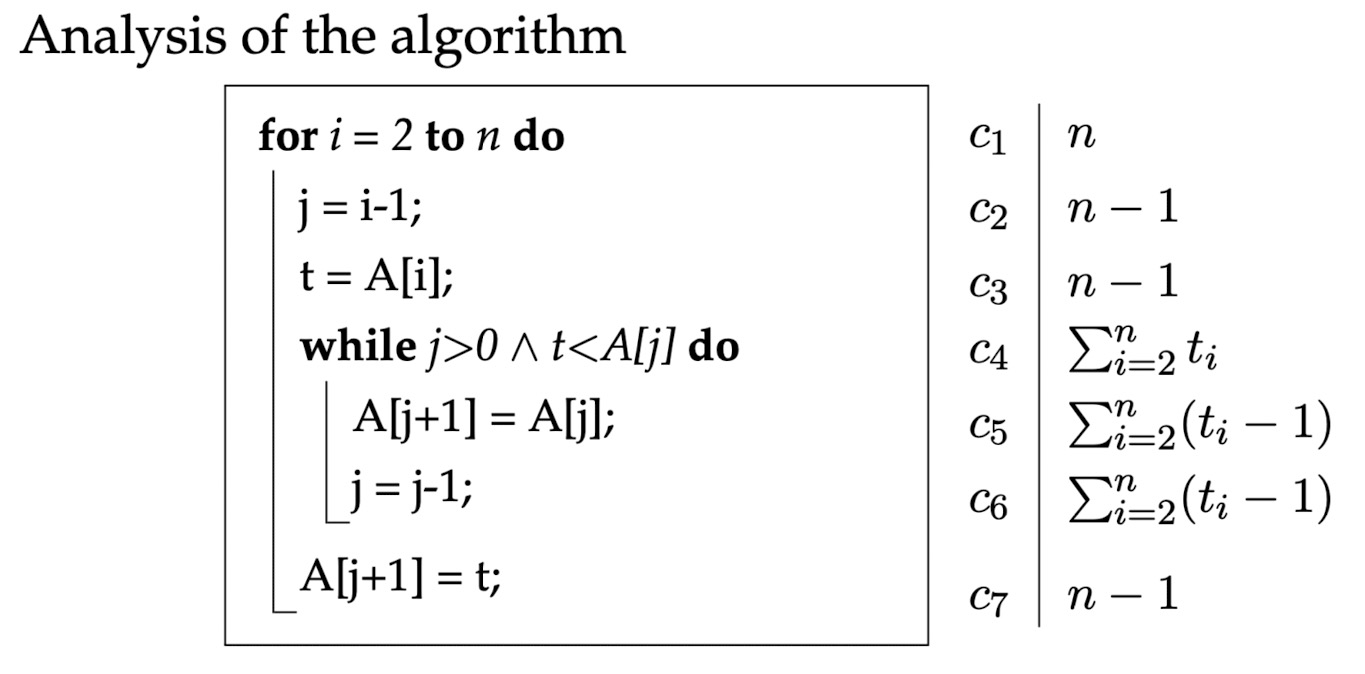
\includegraphics[width=0.5\linewidth]{images/Screenshot 2024-05-24 at 13.57.47.jpg}
\end{figure}

Exact running time: Sum of products (cost, times) \[
T(n)=c_1n + c_2(n-1)+c_3(n-1)+c_4\sum_{i=2}^n t_i + c_5 \sum_{i=2}^n (t_i-1) +c_6 \sum_{i=2}^n (t_i-1)+c_7(n-1)
\]
$\Rightarrow$ Running time as a function of the input size $n$ \\

\textbf{Best case} running time: (Already sorted; $t_i=1$)
\begin{align*}
    T(n)&=c_1n +(c_2+c_3+c_4+c_7)(n-1) \\
    &= \underbrace{(c_1+c_2+c_3+c_4+c_7)}_{a}n -\underbrace{(c_2+c_3+c_4+c_7)}_{b} \\
    &=an+b
\end{align*}
\textbf{Worst case} running time: (Reverse order; $t_i=i$)
\begin{align*}
    T(n)&=c_1n+(c_2+c_3+c_7)(n-1)+c_4\left (\frac{n(n+1)}{2} -1 \right) + (c_5+c_6) \frac{(n-1)n}{2} \\
    &= an^2+bn+c
\end{align*}
\begin{itemize}
    \item In depth explanations of terms:
    \begin{itemize}
        \item $n$ = amount of times the outer loop condition is being checked 
        \item $n-1$ = times the outer loop runs
        \item $\frac{n(n+1)}{2}-1$ = the amount the inner loop condition is being checked
        \begin{itemize}
            \item In the first iteration, we have to compare $n$ elements, thus make $n-1$ comparisons $\Rightarrow$ Inner loop runs $n-1$ times and condition is being checked one time more, thus $n$ times
            \item But as the outer loop runs from $i=2$, the loop $i=1$ is never run. This mean the inner condition is being checked: $n+(n-1)+\cdots+2$ times 
            \item In order to calculate sum of the arithmetic series $\sum_{i=2}^n i$, we have to look at $\sum_{i=1}^n i-1$, thus we get $\frac{n(n+1)}{2} - 1$. [\ref{ARSeries}]
        \end{itemize}
    \end{itemize}
\end{itemize}

\subsubsection{Best, Worst and Average Case: Concluding Remarks}
\begin{itemize}
    \item Often, counting the number of iterations of the core (innermost) part is sufficient
    \begin{itemize}
        \item No distinction between comparisons, assignments, etc.
        \item Means that each of them has roughly the same cost
        \item Does provide results with good/adequate precision
    \end{itemize}
    \item In certain cases the cost of a specific operation may dominate all other costs
    \begin{itemize}
        \item Example: disk I/O versus RAM operations
    \end{itemize}
\end{itemize}

\noindent
\textbf{\underline{Example: Runtime of Binary Search}} \\
\bigskip

\begin{center}
\begin{minipage}{0.6\textwidth}
\begin{algorithm}[H]
\caption{LinSearch(A, v)}
\textbf{Input:} sequence $A[1..n]$ of length $n$, value $v$ \\
\textbf{Output:} either index $i$ such that $v = A[i]$ or $\text{NIL}$ \\
$i = 1$ \\
\While{$i \leq n \land A[i] \neq v$} {
    $i = i + 1$\;}
\If{$i \leq n$} {
     \textbf{return} $i$\;
     }
\Else {
     \textbf{return} $\text{NIL}$\;
     }
\end{algorithm}
\end{minipage}
\end{center}
\begin{itemize}
    \item Running times of Linear Search:
    \begin{itemize}
    \item Worst case: $n$
    \item Average case: $\frac{n}{2}$
    \item Best case: 0
\end{itemize}
\end{itemize}


\begin{center}
\begin{minipage}{0.6\textwidth}
\begin{algorithm}[H]
\caption{BinSearch1(A, v)}
\KwIn{sequence $A[1..n]$ of length $n$, value $v$}
\KwOut{either index $i$ such that $v == A[i]$ or \text{NIL}}
$l = 1$; $r = n$\;
$m = \lfloor (l + r) / 2 \rfloor$\;
\While{$l \leq r$ $\land$ $v \neq A[m]$}{
    \uIf{$v < A[m]$}{
        $r = m - 1$\;
    }
    \Else{
        $l = m + 1$\;
    }
    $m = \lfloor (l + r) / 2 \rfloor$\;
}
\If{$l \leq r$} {
    \Return $m$\;
}
\Else{
    \Return \text{NIL}\;
}
\end{algorithm}
\end{minipage}

\end{center}

Analysis of algorithm:
\begin{itemize}
    \item How many times is the loop executed?
    \begin{itemize}
        \item $log_2n$ - better than linear $n$
    \end{itemize}
\end{itemize}

\subsection{Correctness}

Pre/post-conditions:
\begin{itemize}
    \item \textbf{Assertion}: statement about the state of execution
    \item To prove partial correctness one associates a number of assertions with specific checkpoints in the algorithm
    \item \textbf{Preconditions}: assertions that must be valid before the execution of an algorithm or a subroutine (input)
    \item \textbf{Postconditions}: assertions that must be valid after the execution of an algorithm or a subroutine (output)
\end{itemize}
Loop invariants:
\begin{itemize}
    \item To show correctness of loop statements
    \item \textbf{Invariants}: assertions that are valid any time they are reached
    \item One must show three things about loop invariants 
    \begin{enumerate}
        \item Initialization: it is true before the first iteration
        \item Maintenance: if it is true before an iteration then it is true after that iteration
        \item Termination: when the loop terminates, it gives a useful property that helps to show that the algorithm is correct 
    \end{enumerate}
\end{itemize}

\subsubsection{Correctness of Binary Search}

Invariant: 
\begin{itemize}
    \item $\forall i \in [1..l-1]:v>A[i]$, and
    \item $\forall i \in [r+1..n]:y < A[i]$
    \item In words: elements to the left (right) of $l$ ($r$) are smaller (larger) than v 
\end{itemize}

\textbf{Initialization}: $l=1,r=n$ \\
The invariant holds because there are no elements to the left or right of $l$ and $r$ respectively.
\begin{itemize}
    \item $l=1$ yields $\forall i \in [1..0]:A[i] < v$. This holds since the range [1..0] is empty
    \item $r=n$ yields $\forall i \in [n+1..n]:A[i]>v$. This holds since the range [n+1..n] is empty
\end{itemize}
\textbf{Maintenance}: $l,r,m = \lfloor (l+r)/2 \rfloor $\\
Two cases:
\begin{itemize}
    \item We have $A[m]\neq v, A[m] > v, r=m-1 $, A is sorted. This implies $\forall k \in [r+1..n]:A[k]>v$
    \item We have $A[m] \neq v, A[m] < v, l=m+1 $, A is sorted. This implies $\forall k \in [1..l-1]:A[k]<v $
\end{itemize}

\textbf{Termination}: $l,r,l \leq r$\\
Two cases:
\begin{itemize}
    \item $l=m+1$ allows to conclude $\lfloor(l+r)/2\rfloor +1 >l $
    \item $r=m-1$ allows to conclude $\lfloor(l+r)/2\rfloor -1 < r $
\end{itemize}
Thus, the range gets smaller during each iteration and the loop will terminate when $l\leq r$ no longer holds

\subsubsection{Correctness of Insertion Sort}
Outer loop:
\begin{itemize}
    \item $A[1..i-1]$ is sorted
    \item $A[1..i-1[ \in A^{orig}$ 
\end{itemize}
Inner loop:
\begin{itemize}
    \item $A[i..j],t,A[j+1...i-1]$
    \item $t<A[k]$ for $j+1\leq k \leq i-1$
    \item $A[i..j] \circ A[j+1...i-1]$ sorted
\end{itemize}

\textbf{Initialization}
\begin{itemize}
    \item $i=2$: invariant holds; $A[1..1]$ is trivially sorted 
    \item $j= i-1: A[1..i-1],t,A[i..i-1],t=A[i]$
    \item[] $A[i..i-1]$ is empty (and thus trivially sorted)
    \item[] $A[1..i-1]$ is sorted (invariant of outer loop) 
\end{itemize}

\textbf{Maintenance}
\begin{itemize}
    \item $A[1..i-1]$ is sorted + insert $A[i]$ implies $A[1..i]$ is sorted
    \item $A[1..j-1],t,A[j,j+1..i-1]$ satisfies condition since
    \item[] $A[j]>t $ and $A[1..i-1] $ is sorted
\end{itemize}

\textbf{Termination}
\begin{itemize}
    \item outer loop: $i=n+1$ and $A[1..n]$ is sorted
    \item $A[j]\leq t:A[1..j],t,A[j+1..i-1]=A[1..i] $ is sorted
    \item $j=0: A[t,1..i-1] = A[1..i]$ is sorted
\end{itemize}

\subsection{Asymptotic Complexity}

Asymptotic Analysis
\begin{itemize}
    \item Goal: simplify the analysis of running time
    \item Approach: getting rid of unnecessary details
    \item Fundamental concern: how the running time increases with the size of the input in the limit
\end{itemize}

\subsubsection{Order of Growth}
\textbf{Big-$O$ notation:}
\begin{itemize}
    \item Asymptotic upper bound
    \item Used for \textbf{worst-case analysis}
    \item $f(n)$ and $g(n)$ are function over non-negative integers
    \item $f(n)= O(g(n))$ if and only if there exists constants $c>0$ and $n_0>0$ such that $f(n9 \leq cg(n)$ for $n\geq n_0$
    \item Example proofs:
    \begin{itemize}
        \item $2^{n+1} = O(2^n)$
        \begin{align*}
            2^{n+1} &\leq c\cdot 2^n \\
            2\cdot 2^n &\leq c\cdot 2^n\\
            2&\leq c\\
            \text{holds for } c&\geq 2
        \end{align*}
    \end{itemize}
\end{itemize}
\textbf{Big-$\Omega$ notation}
\begin{itemize}
    \item Asymptotic lower bound
    \item Used for best-case analysis
    \item $f(n) =\Omega(g(n))$ if and only if there exist constants $c>0$ and $n_0>0$ such that $cg(n) \leq f(n) $ for $n\geq n_0$
\end{itemize}

\textbf{Big-$\Theta$ notation}
\begin{itemize}
    \item Asymptotic tight bound
    \item $f(n)= \Theta(g(n))$ if and only if there exist constants $c_1 >0$, $c_2>0$, and $n_0>0$ such that $c_1g(n)\leq f(n) \leq c_2g(n)$ for $n \geq n_0$
    \item $f(n) = \Theta(g(n))$ iff $f(n) = O(g(n))$ and $f(n) = \Omega(g(n))$
\end{itemize}

Useful analogy:
\begin{itemize}
    \item $f(n)=O(g(n)) \quad \leftrightarrow f \leq g $
    \item $f(n)=o(g(n)) \quad \leftrightarrow f < g$
    \item $f(n)=\Omega(g(n)) \quad \leftrightarrow f \geq g$
    \item $f(n)=\omega (g(n)) \quad \leftrightarrow f>g$
    \item $f(n) = \Theta(g(n)) \quad \leftrightarrow f=g$
\end{itemize}


\subsection{Special case analysis}
Basic approach for checking the correctness of a program with special case analysis:
\begin{itemize}
    \item Consider all possible extreme cases
    \item Make sure the solution works in these cases
    \item Problem is reduced to identifying all the special cases 
\end{itemize}

Special cases:
\begin{itemize}
    \item Data structure: empty, single element, completely filled, duplicates, etc.
    \item Particular values, border of domain: Zero, empty string, negative numbers, etc.
    \item Calling of functions (procedures): entering function, termination of function
    \item Control and loop statements: start of loop, end of loop, 1st iteration
\end{itemize}